\subsection{Data reduction analysis} 
\label{sec:dedup_ratio}

\paragraph{Layer sharing}

In its simplest implementation Docker would not support layer sharing.
%
Instead, every image would be a single flat archive.
%
In fact, some existing containerization frameworks
~\cite{singularity}~\cite{openvz} 
%
\VT{cite singularity and openvz}
%
\NZ{addressed}
%
\VT{No, not addressed, citation for singularity is still missing}
%
use flat images.
%
Our estimates show that without layer sharing Docker Hub dataset would grow
from 47TB to 85TB, implying \textbf{1.8$\times$} deduplication ratio provided
by the layer sharing technique.
 
We further computed for each layer, how many times it is referenced by images.
%
Figure~\ref{fig:ref_count} shows that around 90\% of layers are referenced by
only a single image, additional 5\% are referenced by 2 images, and less than
1\% of the layers are shared by more than 25 images.
%
Interestingly, there is one layer that is referenced by 184,171 images.  Our
analysis revealed that this is an empty layer.
%
\VT{Explain the reason for empty layer.}
%
\VT{I feel we might need to talk about 2 more "most referenced" layers.}
%
\VT{Use \% instead of probability in all Figures (both  \# and labels).
We use \% in the text, so we MUST do it.}


\begin{figure}[t]
	\centering
		\begin{minipage}{0.2\textwidth}
			\centering
			\includegraphics[width=1\textwidth]{graphs/shared-cnt-cdf.pdf}
			\caption{CDF of layer reference count.}
			\label{fig:ref_count}
		\end{minipage}
	\begin{minipage}{0.22\textwidth}
		\centering
		\includegraphics[width=1\textwidth]{graphs/layer-size-cdf.pdf}
		\caption{CDF of compress. and uncompress. layer size.}
		\label{fig:layer-size-cdf}
	\end{minipage}%
\end{figure}
%%		\vcomment{Figures \ref{fig:layer-size-cdf} and \ref{fig:compress-ratio}
%have different sizes, looks not neat, please fix.}
%\begin{figure}
%	\centering
%	\includegraphics[width=0.21\textwidth]{graphs/shared-cnt-cdf.pdf}
%	\caption{CDF of layer reference count.
%	}
%	\label{fig:ref_count}
%\end{figure}

\paragraph{Compression}
%
Figure~\ref{fig:layer-size-cdf} presents compressed and uncompressed layer size
distributions.
%
We find that 50\% of the layers are less than 1MB and 90\% of the layers are
less than 64MB in compressed format.
%
If uncompressed, 50\% of the layers are smaller than 2 MB and 90\% of the
layers are smaller than 170MB.
%
Moreover, the total compressed layer dataset grows from 47~TB to 167~TB after decompression, resulting in \textbf{3.6$\times$} compression ratio.

\paragraph{File-level deduplication}
%
Next, we calculate deduplication ratio in terms of file count and capacity for
the complete uncompressed dataset.
%
After removing redundant files, there are only 3.17\% of files left that occupy
23.92~TB, resulting in deduplication ratios of \textbf{31.55$\times$} and
\textbf{6.99$\times$} in terms of file count and capacity, respectively.
%
\begin{figure} \centering
	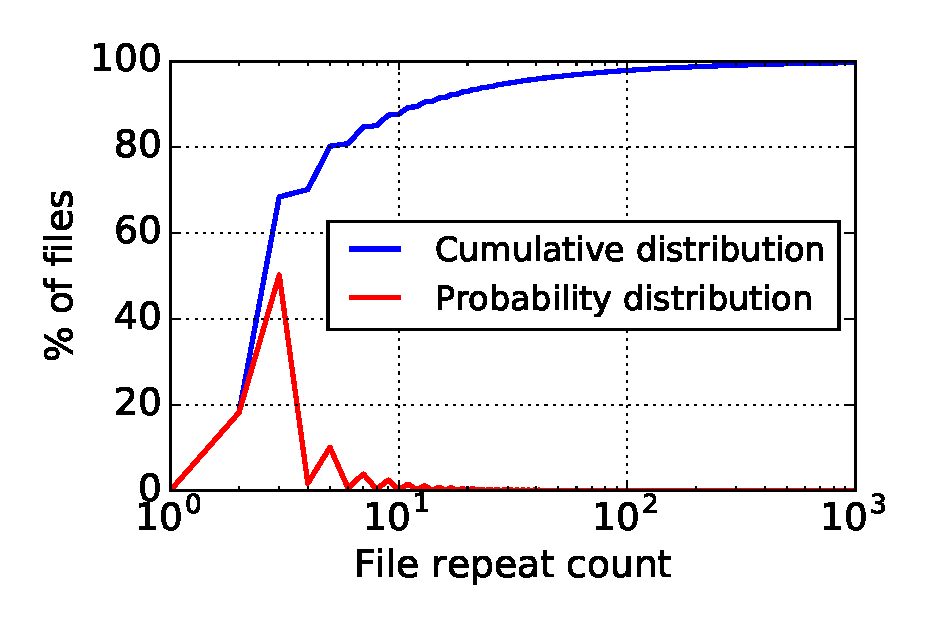
\includegraphics[width=0.45\textwidth]{graphs/File_repeat_count.eps}
	\caption{File repeat count distribution.
	%
	\VT{No need for Y2}
	%
	\VT{Still need to use \% on the axis}
	%
	} \label{fig:file-repeat-cnt}
\end{figure}

%
We further analyzed the repeat count for every file.
%
Figure~\ref{fig:file-repeat-cnt} shows the distributions of file repeat count.  
%
We see that over 99.42\% of files have more than one copy.
%
Around 50\% of files have exactly 4 copies and 90\% of files have 10 or less
copies. 
%
The file that has the maximum repeat count 53,654,306---is an empty file.
%
\VT{Do we know anything about those empty files}.
%
\VT{I believe we need to talk about over frequent files. Maybe in the text
section.}.
